% This file was created by matplotlib2tikz v0.6.18.
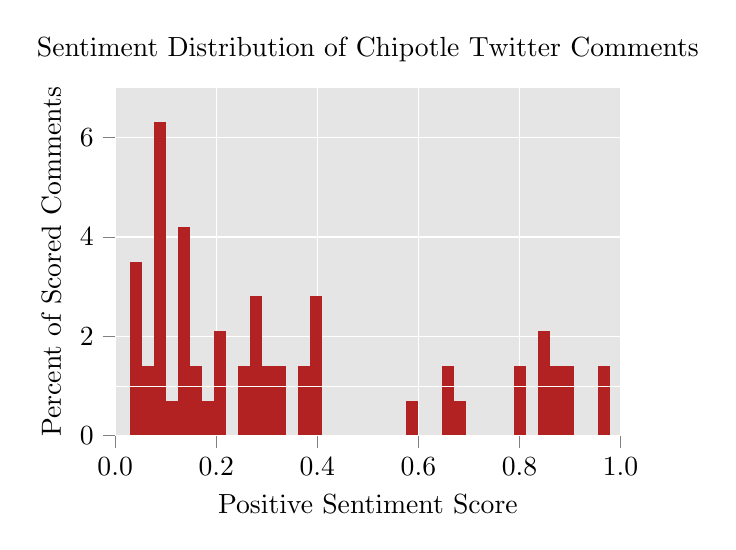
\begin{tikzpicture}

\definecolor{color0}{rgb}{0.698039215686274,0.133333333333333,0.133333333333333}

\begin{axis}[
axis background/.style={fill=white!89.80392156862746!black},
axis line style={white},
height=6cm,
tick align=outside,
tick pos=left,
title={Sentiment Distribution of Chipotle Twitter Comments},
width=8cm,
x grid style={white},
xlabel={Positive Sentiment Score},
xmajorgrids,
xmin=0, xmax=1,
xtick={0,0.2,0.4,0.6,0.8,1},
xticklabels={0.0,0.2,0.4,0.6,0.8,1.0},
y grid style={white},
ylabel={Percent of Scored Comments},
ymajorgrids,
ymin=0, ymax=7
]
\draw[fill=color0,draw opacity=0] (axis cs:0.0286780297756195,0) rectangle (axis cs:0.0524546727538109,3.50484016645113);
\draw[fill=color0,draw opacity=0] (axis cs:0.0524546690285206,0) rectangle (axis cs:0.0762313157320023,1.40193606658045);
\draw[fill=color0,draw opacity=0] (axis cs:0.0762313157320023,0) rectangle (axis cs:0.100007958710194,6.30871229961203);
\draw[fill=color0,draw opacity=0] (axis cs:0.100007951259613,0) rectangle (axis cs:0.123784594237804,0.700968033290226);
\draw[fill=color0,draw opacity=0] (axis cs:0.123784609138966,0) rectangle (axis cs:0.147561252117157,4.20580951766175);
\draw[fill=color0,draw opacity=0] (axis cs:0.147561237215996,0) rectangle (axis cs:0.171337887644768,1.40193562727393);
\draw[fill=color0,draw opacity=0] (axis cs:0.171337872743607,0) rectangle (axis cs:0.195114508271217,0.700968252943626);
\draw[fill=color0,draw opacity=0] (axis cs:0.195114523172379,0) rectangle (axis cs:0.218891173601151,2.10290344091089);
\draw[fill=color0,draw opacity=0] (axis cs:0.218891173601151,0) rectangle (axis cs:0.242667809128761,0);
\draw[fill=color0,draw opacity=0] (axis cs:0.2426677942276,0) rectangle (axis cs:0.266444444656372,1.40193650588725);
\draw[fill=color0,draw opacity=0] (axis cs:0.266444444656372,0) rectangle (axis cs:0.290221095085144,2.80387125454786);
\draw[fill=color0,draw opacity=0] (axis cs:0.290221095085144,0) rectangle (axis cs:0.313997745513916,1.40193562727393);
\draw[fill=color0,draw opacity=0] (axis cs:0.313997745513916,0) rectangle (axis cs:0.337774366140366,1.40193738450168);
\draw[fill=color0,draw opacity=0] (axis cs:0.337774366140366,0) rectangle (axis cs:0.361551016569138,0);
\draw[fill=color0,draw opacity=0] (axis cs:0.361551016569138,0) rectangle (axis cs:0.38532766699791,1.40193562727393);
\draw[fill=color0,draw opacity=0] (axis cs:0.38532766699791,0) rectangle (axis cs:0.409104317426682,2.80387125454786);
\draw[fill=color0,draw opacity=0] (axis cs:0.409104287624359,0) rectangle (axis cs:0.432880908250809,0);
\draw[fill=color0,draw opacity=0] (axis cs:0.432880938053131,0) rectangle (axis cs:0.456657588481903,0);
\draw[fill=color0,draw opacity=0] (axis cs:0.456657588481903,0) rectangle (axis cs:0.480434238910675,0);
\draw[fill=color0,draw opacity=0] (axis cs:0.480434238910675,0) rectangle (axis cs:0.504210889339447,0);
\draw[fill=color0,draw opacity=0] (axis cs:0.504210889339447,0) rectangle (axis cs:0.527987539768219,0);
\draw[fill=color0,draw opacity=0] (axis cs:0.527987599372864,0) rectangle (axis cs:0.551764190196991,0);
\draw[fill=color0,draw opacity=0] (axis cs:0.551764130592346,0) rectangle (axis cs:0.575540781021118,0);
\draw[fill=color0,draw opacity=0] (axis cs:0.575540781021118,0) rectangle (axis cs:0.59931743144989,0.700967813636964);
\draw[fill=color0,draw opacity=0] (axis cs:0.59931743144989,0) rectangle (axis cs:0.623094081878662,0);
\draw[fill=color0,draw opacity=0] (axis cs:0.623094081878662,0) rectangle (axis cs:0.646870732307434,0);
\draw[fill=color0,draw opacity=0] (axis cs:0.646870732307434,0) rectangle (axis cs:0.670647382736206,1.40193562727393);
\draw[fill=color0,draw opacity=0] (axis cs:0.670647382736206,0) rectangle (axis cs:0.694424033164978,0.700967813636964);
\draw[fill=color0,draw opacity=0] (axis cs:0.694424033164978,0) rectangle (axis cs:0.71820068359375,0);
\draw[fill=color0,draw opacity=0] (axis cs:0.71820068359375,0) rectangle (axis cs:0.741977274417877,0);
\draw[fill=color0,draw opacity=0] (axis cs:0.741977274417877,0) rectangle (axis cs:0.765753924846649,0);
\draw[fill=color0,draw opacity=0] (axis cs:0.765753924846649,0) rectangle (axis cs:0.789530575275421,0);
\draw[fill=color0,draw opacity=0] (axis cs:0.789530575275421,0) rectangle (axis cs:0.813307225704193,1.40193562727393);
\draw[fill=color0,draw opacity=0] (axis cs:0.813307225704193,0) rectangle (axis cs:0.837083876132965,0);
\draw[fill=color0,draw opacity=0] (axis cs:0.837083876132965,0) rectangle (axis cs:0.860860526561737,2.10290344091089);
\draw[fill=color0,draw opacity=0] (axis cs:0.860860526561737,0) rectangle (axis cs:0.884637176990509,1.40193562727393);
\draw[fill=color0,draw opacity=0] (axis cs:0.884637236595154,0) rectangle (axis cs:0.908413827419281,1.40193914173383);
\draw[fill=color0,draw opacity=0] (axis cs:0.908413767814636,0) rectangle (axis cs:0.932190418243408,0);
\draw[fill=color0,draw opacity=0] (axis cs:0.932190418243408,0) rectangle (axis cs:0.95596706867218,0);
\draw[fill=color0,draw opacity=0] (axis cs:0.95596706867218,0) rectangle (axis cs:0.979743719100952,1.40193562727393);
\path [draw=white, fill opacity=0] (axis cs:0,0)
--(axis cs:0,7);

\path [draw=white, fill opacity=0] (axis cs:1,0)
--(axis cs:1,7);

\path [draw=white, fill opacity=0] (axis cs:0,0)
--(axis cs:1,0);

\path [draw=white, fill opacity=0] (axis cs:0,1)
--(axis cs:1,1);

\end{axis}

\end{tikzpicture}